% !TeX encoding = UTF-8
\chapter{SDE的数值解法}\label{chap3}

\section{SDE 的收敛阶}

本节考虑随机微分方程(\ref{SDDE}),即系数函数 $b,\sigma$ 不带随机变量 $\omega$. 我们研究这类方程的数值解法的收敛性. 令 $(\Omega,\mF,P)$ 为概率空间,$(w_r(t),\mF_t),r=1,\cdots,m$ 是独立的 Wiener 过程. 考虑 \ito 意义下的随机微分方程:
\begin{equation}\label{eq3.1}
	\md X=b(t,X) \md t+\sum_{r=1}^m \sigma_r(t,X) \md w_r(t),
\end{equation}
这里 $X,b,\sigma_r$ 均为 $d$ 维向量. 且满足上节中的假设 $A$,此时强解存在且唯一. 

依赖于 $x,t,h$ 的单步数值解法,我们记为$\overline{X}_{t,x}(t+h)$,即
\begin{equation}\label{eq3.2}
	\overline{X}_{t,x}(t+h) = x+A(t,x,h;w_i(\theta) - w_i(t),i=1,\cdots,m,t\le \theta \le t+h).
\end{equation}
并将准确解记作 $X_{t,x}(t+h)$ . 使用单步法时,一般将区间 $[0,T]$ 均分为 $N$ 个小区间,$t_0=0,t_k = kh, t_{_N} = T$,这里 $h = \frac TN$. 我们记
\begin{equation}\label{eq3.3}
	\begin{aligned}
	&\overline{X}_0 = X_0 = X(0),\\ 
	&
	\begin{aligned}
		\overline{X}_{k+1} &= \overline X_{t_k,\overline X_k}(t_{k+1})\\
		&=\overline X_k + A(t_k,\overline X_k ,h_{k+1}; w_i(\theta) - w_i(t),i=1,\cdots,m,t\le \theta \le t+h).
	\end{aligned}
	\end{aligned}
\end{equation}
这里 $K=0,1,\cdots,N-1$.下面的定理告诉我们局部截断误差与整体截断误差之间的联系. 
\begin{theorem}\label{thm_3.1}
	假设一个单步法 $\overline X_{t,x}(t+h)$ 在期望意义下有 $p_1$ 阶的偏差,以及 $p_2$ 阶的均方误差.即对于 $t \in [0,h],x \in \R^d$,有
	\begin{equation}\label{eq3.4}
		\begin{aligned}
		\left|{E}\left(X_{t, x}(t+h)-\overline{X}_{t, x}(t+h)\right)\right| \leq K\left(1+|x|^{2}\right)^{1 / 2} h^{p_{1}} \\
		\left.{E}\left|X_{t, x}(t+h)-\overline{X}_{t, x}(t+h)\right|^{2}\right]^{1 / 2} \leq K\left(1+|x|^{2}\right)^{1 / 2} h^{p_{2}}
		\end{aligned}
	\end{equation}
	且 $p_2 \ge \frac12,p_1\ge p_2+\frac12$. 
	则对任意 $k=0,1,2,\cdots,N$,有如下不等式成立:
	\begin{equation}\label{eq3.5}
		\left[E\left|X_{0, X_{0}}\left(t_{k}\right)-\overline{X}_{0, X_{0}}\left(t_{k}\right)\right|^{2}\right]^{1 / 2} \leq K\left(1+E\left|X_{0}\right|^{2}\right)^{1 / 2} h^{p_{2}-1 / 2}
	\end{equation}
	即,利用单步法构造的数值方法 $\overline{X}_{t,x}(t+h)$ 的整体误差阶 $p = p_2-\frac12$. 
\end{theorem}
该定理的证明相当冗长,见文献\cite{book_error}. 但该定理的结论非常实用,仅需证明单步法的局部截断误差估计,就可以得到单步法的整体误差估计. 



\section{单步法}
\subsection{Euler格式}
随机系统 (\ref{eq3.1}) 应用最简单的显式 Euler 格式,形式为
\begin{equation}\label{eq3.6}
	\overline{X}_{t,x}(t+h) = x + b(t,x)h+\sum_{r=1}^{m} \sigma_r(t,x) \Delta_t w_r(h),
\end{equation}
这里 $\Delta_t w_r(h) = w_r(t+h) - w_r(t),\quad r=1,2,\cdots,m$. 
Euler 格式是最基础的单步法,仅具有 $\frac12$ 阶的整体误差,但该结论的证明并不容易. 根据恒等式
\begin{equation}\label{eq3.7}
	X_{t,x}(t+h) = x+\int _t^{t+h} \left( b(s,X_{t,x}) \md s + \sum_{r=1}^m \sigma_r (s,X_{t,x}(s)) \md w_r(s) \right)
\end{equation}
有 
\begin{equation}\label{eq3.8}
	\begin{aligned} 
	X_{t,x}(t+h) - \overline{X}_{t,x}(t+h) =& \int_t^{t+h} \Bigl( b(s,X_{t,x}(s)) - b(t,x) \md s\\
	& + \sum_{r=1}^m  (\sigma_r(s,X_{t,x}(s) -\sigma_r(t,x)) \md w_r(s)) \Bigl)
	\end{aligned} 
\end{equation}
后半部分为鞅,因此误差的期望为
\begin{equation}\label{eq3.9}
	E\left(X_{t,x}(t+h) - \overline{X}_{t,x}(t+h) \right) = 
	E \int_t^{t+h}  b(s,X_{t,x}(s)) - b(t,x) \md s
\end{equation}
同时误差平方的期望为
\begin{equation}\label{eq3.10}
	\begin{aligned}
	E( X_{t,x}&(t+h) - \overline{X}_{t,x}(t+h) ) ^2 = 
		E\left(\int_t^{t+h}  b(s,X_{t,x}(s)) - b(t,x) \md s\right)^2 \\
		&+2E \left(  \int_t^{t+h}  b(s,X_{t,x}(s)) - b(t,x) \md s \sum_{r=1}^m
		 \int_t^{t+h}  b(s,X_{t,x}(s)) - b(t,x) \md w_r(s) \right)\\
		& \qquad\qquad + \sum_{r=1}^m \int_t^{t+h}  E(b(s,X_{t,x}(s)) - b(t,x))^2 \md w_r(s)\\
		& \le  2 E\left(\int_t^{t+h}  b(s,X_{t,x}(s)) - b(t,x) \md s\right)^2  
		 + 2 \sum_{r=1}^m \int_t^{t+h}  E(b(s,X_{t,x}(s)) - b(t,x))^2 \md w_r(s)
	\end{aligned}
\end{equation}
根据预备知识中的线性增长条件和Lipschitz假设,对 $b,\sigma_r$ 有如下估计式:
\begin{equation}\label{eq3.11}
	\begin{aligned}
	\left|  b(s,X_{t,x}(s)) - b(t,x) \right| 
	& \le   |b(s,X_{t,x}(s)) - b(s,x)|+ |b(s,x) - b(t,x)| \\
	& \le   K| X_{t,x}(s) - x| + K \left(1+|x|^2\right)^{1/2} (s-t).
	\end{aligned}
\end{equation}
再由 Cauchy-Bunyakovsky-Schwarz 不等式,有
\[
\left|\int_{t}^{t+h}\left(b\left(s, X_{t, x}(s)\right)-b(t, x)\right) d s\right|^{2} \leq h \int_{t}^{t+h}\left(b\left(s, X_{t, x}(s)\right)-b(t, x)\right)^{2} d s
\]
根据定理3.1的假设,因此(\ref{eq3.10})的第一项可以被 $K(1+|x|^2)h^4$ 控制,而第二项被 $K(1+|x|^2)h^2$ 控制. 根据定理3.1,$p_1=2,p_2=1,p=p_2-\frac12=\frac12$,即 Euler 格式具有 $\frac12$ 阶整体误差. 

\begin{remark}
当扩散项系数仅与 $t$ 有关时,即 SDE 形如
\begin{equation}\label{eq3.12}
	\md X(t) = b(t,X_t) \md t + \sum_{r=1}^m \sigma_r(t) \md w_r(t),
\end{equation}
此时 Euler 格式具有 1 阶整体误差. 
\end{remark}


本文考虑自治随机微分方程(\ref{SODE}),称对应 Euler 格式
\begin{equation}\label{Euler_Maruyama}
	\overline{X}_{t,x}(t+h) = x+b(x)h+\sum_{r=1}^m \sigma_r(x) \Delta_t w_r(h),
\end{equation}
为 Euler-Maruyama 格式,其具有 0.5 阶整体误差精度.

\paragraph*{ 例子}
考虑几何布朗运动模型
\[
 \md X_t = b X_t \md t + \sigma X_t d B_t,
\]
这里 $b$ 和 $\sigma$ 均为常数. 则方程有精确解:
\[
	X_t = X_0 \exp \left[\left(b-\frac12\sigma^2\right)T + \sigma B_T\right]. 
\]
解表现为对数正态分布. 由 $E \exp (B_T) = \exp(T/2)$,其期望和方程分别是:
\[
	E(X_T) = X_0 e^{bT},\qquad D(X_T) = X_0^2 e^{2bT} \left( e^{\sigma^2T}-1 \right).
\]

\begin{figure}[!htbp]
	\centering 
	\subfigure[样本轨迹1]{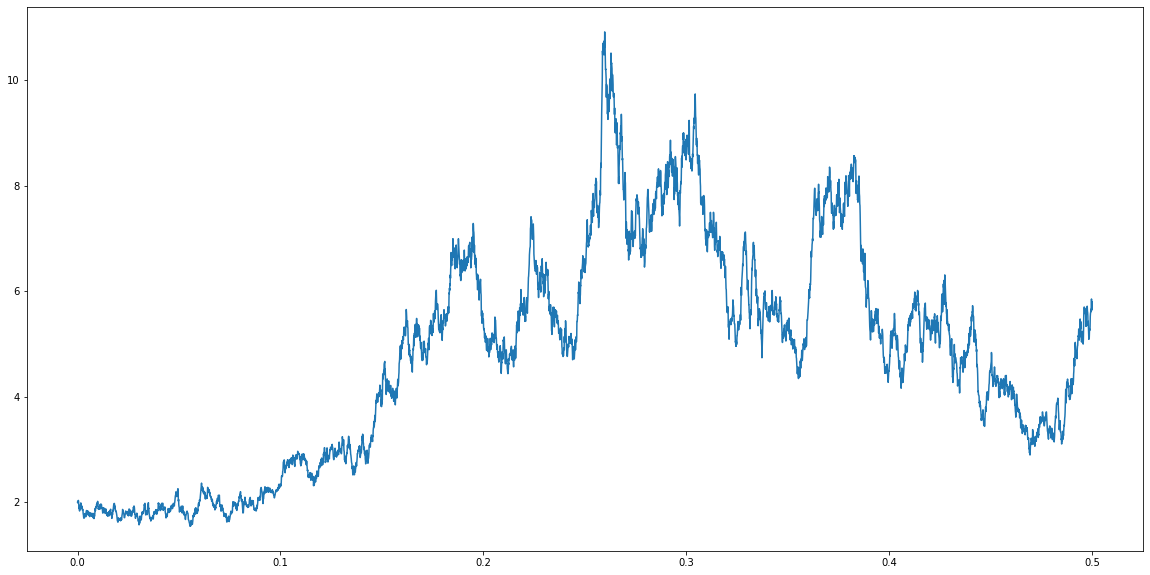
\includegraphics[width=2.95in]{images/path_1}}
	\subfigure[样本轨迹2]{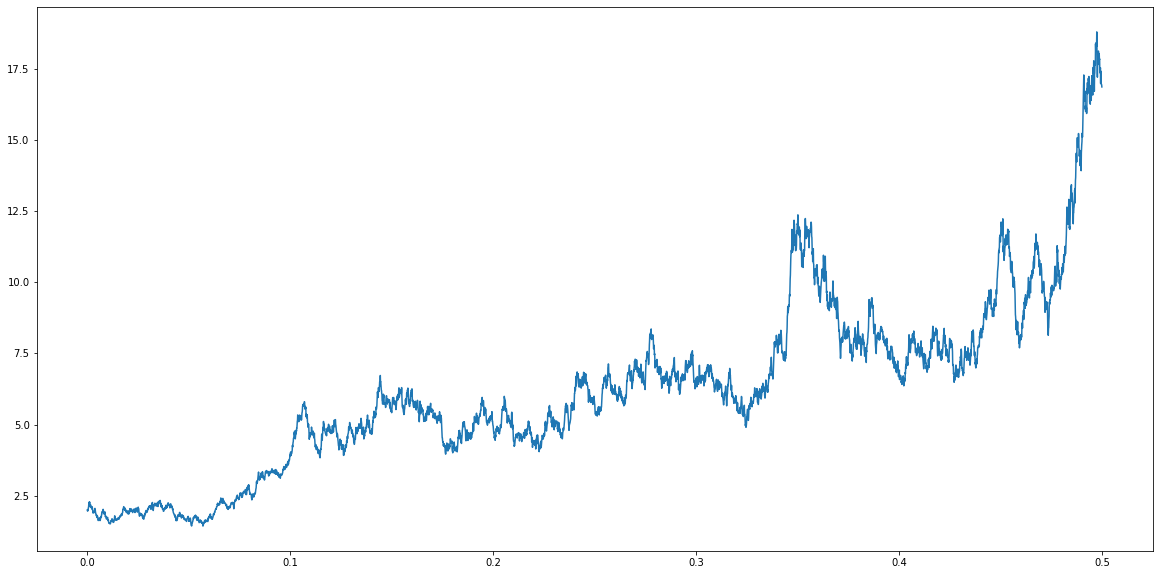
\includegraphics[width=2.95in]{images/path_2}}
	\caption{欧拉方法模拟几何布朗运动} 
	\vspace{.2cm}
	\label{path_1_2}
\end{figure}

一些数值测试表明,欧拉方法在该样例中是可靠的,见表\ref{tab_1},蒙特卡洛模拟的样本轨道数量为 $10^4$. 


\begin{table}[!htbp]
\centering
\begin{tabular}{r|c|c|c|c|c|c|c|c}
	方程参数 & 时间($T$) & $EX$ & $DX$& 步长($h$) & $E\overline X$ & $D\overline X$&$ E|X-\overline X| $   & $E(X-\overline X)^2$  \\
	\hline
	$X_0=2$&&&&             1e-2&2.402&43.00&7.27e-3&12.27 \\
	$b=2$&0.1&2.442&66.72&  1e-3&2.421&53.83&1.88e-3&1.361 \\
	$\sigma=5$&&&&          1e-4&2.425&58.45&5.18e-4&0.137 \\
	\hline
	$X_0=2$&&&&             1e-2&22.68&1911&1.187&117.7 \\
	$b=2$&0.5&24.36&3792&   1e-3&25.30&4634&0.214&31.06 \\
	$\sigma=5$&&&&          1e-4&23.98&4075&0.007&1.605 \\
	\hline
	$X_0=2$&&&&             1e-2&8.14e-5&5.26e-5&1.22e-4&1.37e-3 \\
	$b=2$&3&806.8&inf&      1e-3&5.09e-4&8.45e-4&5.93e-4&1.06e-3 \\
	$\sigma=5$&&&&          1e-4&2.47e-3&3.81e-2&1.57e-3&2.17e-2 \\
	\hline
	$X_0=2$&&&&             1e-2&0.7305&4.587&4.36e-3&0.1312\\
	$b=-2$&0.5&0.7357&3.458&1e-3&0.7454&3.605&2.93e-3&0.0181\\
	$\sigma=2$&&&&          1e-4&0.7165&3.145&6.92e-4&0.0013\\
	\hline
	$X_0=2$&&&&             1e-2&0.2694&1.907&9.73e-3&0.2106\\
	$b=-2$&1&2.707&3.926&   1e-3&0.2820&2.385&1.54e-3&0.0322\\
	$\sigma=2$&&&&          1e-4&0.2547&1.388&2.61e-4&0.0012\\
	\hline
	$X_0=2$&&&&             1e-2&2.26e-5&7.61e-7&1.18e-5&1.34e-6\\
	$b=-2$&5&9.080e-5&4.000&1e-3&1.38e-5&5.49e-8&7.75e-7&1.15e-9\\
	$\sigma=2$&&&&          1e-4&2.14e-5&3.01e-7&7.02e-8&7.0e-10\\
\end{tabular}
\vspace{.2cm}
\caption{欧拉方法的蒙特卡洛模拟} 
\label{tab_1}
\end{table}
注意到表\ref{tab_1}中,$D\overline{X}$ 不一定能收敛到 $DX$,但每条样本轨道上的误差的一阶矩和二阶矩是可以被 $h$ 控制的,且误差阶与上文计算的一致. 同时对 $b-\frac12 \sigma^2>0$ 的情况,时间 $T$ 取的稍大,会解曲线会爆炸增长;相应的,对 $b-\frac12 \sigma^2<0$ 的情况,会收敛到0. 

基于前文叙述的显式 Euler 格式,可以很自然的叙述出相应的隐格式 Euler 算法,此处简略,后文将介绍精度更高的方法,而此处隐格式算法的稳定性的讨论则过于冗长.



\subsection{Taylor  方法}
引入算子记号
\[
\begin{aligned} 
& \Lambda_k = \sigma_k ^ T \frac{\partial }{\partial x}  =  (\sigma_k,\frac{\partial}{\partial x}) = \sum_{i=1}^d \sigma_k^i \frac{\partial}{\partial x^i},\\
& L = \frac{\partial}{\partial t} + b^T \frac{\partial}{\partial x} + \frac12 \sum_{k=1}^m \sum_{i=1}^d \sum_{j=1}^d \sigma_k^i \sigma_k^j \frac{\partial^2}{\partial x^i \partial x^j}.
\end{aligned}
\]
称算子 $L$ 为 Lyapunov 算子. 

借助 \ito 公式和 Taylor 展开,对于光滑二元函数 $f(t,x)$,有
\begin{equation}\label{eq3.14}
f(T,X(T)) = f(t,x(t)) + \sum_{r=1}^m \int_t^T \Lambda_r f(\theta,X(\theta)) \md B_r(\theta) + \int_t^T Lf(\theta,X(\theta)) \md \theta.
\end{equation}
再对于 $\Lambda_rf$ 和 $Lf$ 做类似(\ref{eq3.14})的展开,得二阶展开表达式
\begin{equation}\label{eq3.15}
\begin{aligned}
	f(T,X(T)) = f  &+ \sum_{r=1}^m \Lambda_rf \int_t^T \md B_t(\theta) + Lf\int_t^T\md \theta\\
	&+\sum_{r=1}^m \int_s^T \left( \sum_{i=1}^m \int_t^\theta \Lambda_i\Lambda_r f(\theta_1,X(\theta_1))\md B_i(\theta_1) \right) \md B_r(\theta)\\
	&+\sum_{r=1}^m \int_t^T \left(  \int_t^\theta L\Lambda_r f(\theta_1,X(\theta_1))\md \theta_1\right) \md B_r(\theta) \\
	&+ \sum_{r=1}^m \int_t^T \left(  \int_t^\theta \Lambda_r Lf(\theta_1,X(\theta_1))\md B_r(\theta_1)\right) \md \theta \\
	&+\int_t^T \left( \int_t^\theta L^2 f(\theta_1,X(\theta_1)) \md\theta_1\right)\md \theta
\end{aligned} 
\end{equation}
此处 $f,\Lambda_rf,Lf$ 均指在 $(t,X(t))$ 处的值. 可以继续对于 $L^2f,L\Lambda_r,\Lambda_rL,\Lambda_i\Lambda_r$ 做类似(\ref{eq3.14})的展开,本节不继续赘述. 基于(\ref{eq3.15}), 有
\begin{equation}\label{eq3.16}
\begin{aligned} 
	f(t+h,X(t+h)) = f &+ \sum_{r=1}^m \Lambda_rf\int_t^{t+h} \md B_r(\theta) + Lf \int_t^{t+h} \md \theta \\
	& + \sum_{r=1}^m\sum_{i=1}^m \Lambda_i\Lambda_rf \int_t^{t+h} \md B_r(\theta) \int_t^\theta \md B_i(\theta_1)\\
	& + \sum_{r=1}^m\sum_{i=1}^m\sum_{s=1}^m \Lambda_s\Lambda_i\Lambda_r f
	\int_t^{t+h}\md B_r(\theta) \int_t^\theta \md B_i(\theta_1) \int_t^{\theta_1} \md B_s(\theta_2)\\
	&+\sum_{r=1}^m \Lambda_rLf \int_t^{t+h} \md \theta \int_t^\theta \md B_r(\theta_1)
	 +\sum_{r=1}^m L\Lambda_rf \int_t^{t+h} \md B_r(\theta) \int_t^\theta \md \theta_1\\
	&+L^2f\int_t^{t+h} \md \theta \int_t^\theta\md \theta_1 + R 
\end{aligned}
\end{equation}
$R$ 表示高阶项.取 $f(t,x)=x$,则有
\[
\Lambda_rf = \sigma_r,\qquad Lf=b.
\]
并计算积分式,带入(\ref{eq3.16})得 Taylor 方法:
\begin{equation}\label{eq_taylor}
\begin{aligned}
\overline{X}_{t,x} (t+h) = x &+ bh+\sum_{r=1}^m \sigma_r(B_r(t+h)-B_r(t))\\
	&+\sum_{r,i=1}^m \Lambda_i\sigma_r \left( \frac12 (B_r(t+h) - B_r(t))^2 - \frac 12 h \right)\\
	&+\sum_{r=1}^m \Lambda_rb \int_t^{t+h} B_r(\theta)-B_r(t) \md \theta\\
	&+\sum_{r=1}^m L\sigma_r  \int_t^{t+h} (\theta - t)\md B_r(\theta)\\
	&+\sum_{r,i,s=1}^m \Lambda_s\Lambda_i\sigma_r \int_t^{t+h} \left(
	  \int_t^\theta B_s(\theta_1) - B_s(t) \md B_i(\theta_1)\right)\md B_r(\theta)\\
	&+\frac{Lbh^2}{2}
\end{aligned}
\end{equation}
对 $X_{t,x}(t+h)$ 的这种展开,也称为 Wagner-Platen 展开. 注意到存在无法精确计算的积分式,因此实际操作的时候,会引入数值积分并引入进一步的误差. 

\paragraph*{ 例子} 考虑线性随机微分方程系统
\begin{equation}\label{eq3.18}
	\md X = A(t) X \md t + \sum_{r=1}^m B_r(t) X\md B_r(t),\qquad  t\in [0,T].
\end{equation}
这里 $A(t),B_r(t)$ 均为 $d\times d$ 的矩阵函数. 由
\[
\Lambda_i\sigma_r(t,x) = B_i(t) x\times \frac{\partial}{\partial x} (B_r(t)x) = B_r(t)B_i(t)x.
\]
其余项在算子作用下变成0,因此数值格式为:
\[
\begin{aligned} 
	\overline{X}_{t,x}(t+h) =x&+\sum_{r=1}^m B_r(t) x \Delta_tB_r(h) + A(t)x h 
	+ \frac12\sum_{r=1}^m B_r^2(t) x (\Delta_t^2 B_r(h)-h)\\
	&+\sum_{r=2}^m\sum_{i=1}^{r-1} B_i(t)B_r(t) x \Delta_t B_i(h) \Delta_t B_r(h).
\end{aligned}
\]
在这个例子中,包含 $m$ 个布朗运动,需要特别注意 $B_i,B_j$ 在 $i\neq j$ 时相互独立,而在 $i=j$ 时,协方差非零. 


对于自治随机微分方程,函数 $b,\sigma$ 是仅关于 $x$ 的函数. 此处介绍一种 Taylor 格式,其具有$\frac32$阶的整体误差精度.
\begin{equation}\label{Taylor}
\begin{aligned}
\overline{X}_{t,x} (t+h)=& x+h b + \sigma \Delta_B +\frac12 \sigma'\sigma (\Delta_B^2-h) + \frac12 \left( b'b + \frac 12 b''\sigma^2 \right) h^2\\
&+\frac{1}{2}(b'\sigma)
\left(\Delta _B +\frac{1}{\sqrt{3}} \int _t^{t+h} B_\theta \md \theta\right) h\\
&+\frac{1}{2}\left( \sigma'b+\frac12 \sigma ''\sigma^2 \right)
\left(\Delta _B - \frac{1}{\sqrt{3}} \int _t^{t+h} B_\theta \md \theta\right) h\\
&+\frac16 (\sigma'^2 \sigma + \sigma''\sigma^2) (\Delta_B^3-3h\Delta _B)
\end{aligned}
\end{equation}
对于一些构造良好的例子,数值格式(\ref{Taylor})中不可精确积分的表达式正好可以消去,从而得到可以显式数值格式. 




\subsection{Milstein 格式 、中点公式、隐格式}
Milstein 格式是特殊的Taylor方法,对于自治随机微分方程(\ref{SODE}),有 $\Lambda_ig_r = \Lambda_rg_i$,称数值格式为
\[
\begin{aligned} 
	\overline{X}_{t,X}(t+h) = x+&f(x)h + \sum_{r=1}^m g_r(x) \Delta_t B_r(h) - \frac12\sum_{r=1}^m \Lambda_rg_r(x)[ (\Delta_t B_r(h))^2-h] \\
	+&\sum_{i=1}^m \sum_{r=i+1}^m\Lambda_ig_r(x) \Delta_t B_i(h) \Delta_t B_r(h).
\end{aligned} 
\]
Milstein 格式,其中 $\Lambda_ig_r(x) = (g_r(x))^Tg_i(x)$. Milstein 格式具有1阶整体误差精度. 

%\subsection{中点公式}
自治随机微分方程(\ref{SODE})的中点格式为
\begin{equation}\label{mid_point}
\overline{X}_{t,x}(t+h) = x + b\left( \frac{x+\overline{X}}{2}\right) h  - \frac12 \sum^q_{r=1} \frac{\partial \sigma_r}{\partial x} \sigma_r \left( \frac{x+\overline{X}}{2}\right) h  + \sum^q_{r=1} \sigma_r \left(\frac{x+\overline X}{2} \right)  \Delta_t B_r(h),
\end{equation}
在线性增长条件和 Lipschitz 条件成立的情况下,中点公式具有1阶整体误差精度,见文献\cite{kutta_1,kutta_2}. 中点公式是隐格式,一般具有更好的数值稳定性. 但相对应的,其向前的差分往往不能直接导出,数值实现会复杂一些. 

文献\cite{Implicit_Taylor,Implicit_Taylor_1,Implicit_Taylor_2}给出了自治随机微分方程(\ref{SODE})的半隐 Milstein 格式和半隐 Taylor格式,见(\ref{eq3.20}). 可以看出这两种隐格式与对应的显格式几乎是一致的,仅是取点有所不同. 同样的数值精度下,具体选择哪种格式则依据实际需求. 本文第5节介绍的保守恒量的数值格式全部为隐格式, 
\begin{equation}\label{eq3.20}
\begin{aligned}
x_{n+1} = x_n+&b(x_{n+1})h + \sigma(x_n) \Delta B + \frac12 [\sigma^\prime \sigma] (x_n) ((\Delta B)^2-h) \\
x_{n+1} = x_n+&b(x_{n+1})h + \sigma(x_n) \Delta B + \frac12 [\sigma^\prime \sigma] (x_n) ((\Delta B)^2-h)\\
			 +&\frac{1}{2} [b^{\prime} \sigma](x_n)\left(\frac{\Delta B'}{\sqrt{3}}-\Delta B\right)h
			 -\frac{1}{2}\left[b^{\prime} b+\frac{1}{2} f^{\prime \prime} \sigma^{2}\right](x_{n+1}) h^2\\
			 +&\frac12\left[\sigma^{\prime} +\frac12 \sigma^{\prime \prime} \sigma^{2}\right](x_n)\left(\Delta B-\frac{\Delta B'}{\sqrt{3}}\right) h\\
			 +&\frac{1}{6}\left[\sigma^{\prime 2} \sigma+\sigma^{\prime \prime} \sigma^{2}\right](x_n) (\left(\Delta B\right)^3-3 h \Delta B )
\end{aligned}
\end{equation}
这里的 $\displaystyle \Delta_B' = \frac{1}{\sqrt{3}} \int _t^{t+h} B_\theta \md \theta$,由于随机分析中的等距公式,其服从均值为0、方差为 $\frac13$ 的正态分布. 
自治随机微分方程的半隐 Milstein 格式和半隐 Taylor格式分别具有1阶和 $\frac32$阶的整体误差. 


\section{多步法}

%\subsection{Runge-Kutta 方法}
此处仅介绍一维自治随机微分方程(\ref{SODE})的随机 Runge-Kutta 方法,更一般问题的多步法见文献\cite{book_kutta}.

s步Runge-Kutta方法定义如下:
\begin{equation}\label{kutta}
\begin{aligned}
X_{n+1} = X_n + & \sum_{i=1}^s \alpha_i b(H_i^{(0)}) h + \sum_{i=1}^s\gamma_i^{(1)} \sigma(H_i^{(1)})\Delta_tB \\
+ & \sum_{i=1}^s \gamma_i^{(2)} \sigma(H_i^{(1)})\frac1{\sqrt h} \int_t^{t+h}\md B(\theta_1) \int_t^{\theta_1} \md B(\theta)
\end{aligned}
\end{equation}
其中
\[
\begin{aligned}
H_{i}^{(0)} &=X_{n}+\sum_{j=1}^{i-1} A_{i j}^{(0)} b\left(H_{j}^{(0)}\right) h+\sum_{j=1}^{i-1} B_{i j}^{(1)^{(0)}} \sigma\left(H_{j}^{(1)}\right) \Delta_tB \\
H_{i}^{(1)} &=X_{n}+\sum_{j=1}^{i-1} A_{i j}^{(1)} b\left(H_{j}^{(0)}\right) h+\sum_{j=1}^{i-1} B_{i j}^{(3)^{(1)}} \sigma\left(H_{j}^{(1)}\right) \sqrt{h}
\end{aligned}
\]
使用 Butcher-Arrays 形式表示 
\begin{table}[!htbp]
\centering
\begin{tabular}{p{1cm}<{\centering} | p{2cm}<{\centering} | p{2cm}<{\centering} |p{2cm}<{\centering}}
	\multirow{2}{*}{} & $A^{(0)}$ & $B^{(1)^{(0)}}$ & \\
	\cline{2-4}
	\rule{0pt}{13pt} & $A^{(1)}$ & $B^{(3)^{(1)}}$ & \\
	\hline
	\rule{0pt}{15pt} $(p_{_D} , p_{_S})$& $\alpha^T$ & $\gamma^{(1)^T}$ & $\gamma^{(2)^T}$\\
\end{tabular}
\end{table}
这些参数需要满足28个方程\cite{book_kutta}. 
即使对于确定性的微分方程,Runge-Kutta 格式系数的计算也相当繁琐,而对于随机微分方程,则计算复杂度更是大大提升. 
这里直接介绍两种解:
\begin{table}[!htbp]
	\centering
	\begin{tabular}{p{1cm}<{\centering} | p{2.5cm}<{\centering} | p{2.5cm}<{\centering} |p{2cm}<{\centering}}
		\multirow{2}{*}{}
		\rule{0pt}{30pt} &  
		$\begin{matrix}	&&A^{(0)}\\\frac23 &&\\-\frac13&1& \end{matrix}$& 
		$\begin{matrix} &&B^{(1)^{(0)}} \\ 1&&\\0&0&  \end{matrix}$ & \\
		\cline{2-4}
		\rule{0pt}{30pt} & 
		$\begin{matrix} &&A^{(1)} \\ 1&&\\1&0& \end{matrix}$ & 
		$\begin{matrix} &&B^{(3)^{(1)}} \\ 1&&\\-1&0&\end{matrix} $ & \\
		\hline
		\rule{0pt}{15pt} $(3,2)$ &  
		$\begin{matrix} \frac14&\frac12&\frac14 &  \end{matrix}$ & 
		$\begin{matrix} \frac12&\frac14&\frac14 ~& \end{matrix}$ & 
		$\begin{matrix} 0&\frac12&-\frac12   \end{matrix}$\\
	\end{tabular}
\vspace{.2cm}
\caption{SRK 格式一} \label{SRK1}
\end{table}
\begin{table}[!htbp]
	\centering
	\begin{tabular}{p{1cm}<{\centering} | p{2.5cm}<{\centering} | p{2.5cm}<{\centering} |p{2cm}<{\centering}}
		\multirow{2}{*}{}
		\rule{0pt}{30pt} &  
		$\begin{matrix}	&&A^{(0)}\\\frac23 &&\\-\frac12&\frac12& \end{matrix}$& 
		$\begin{matrix} &&B^{(1)^{(0)}} \\ 0&&\\1&0&  \end{matrix}$ & \\
		\cline{2-4}
		\rule{0pt}{30pt} & 
		$\begin{matrix} &&A^{(1)} \\ \frac14&&\\0&\frac14& \end{matrix}$ & 
		$\begin{matrix} &&B^{(3)^{(1)}} \\ -\frac12&&\\\frac12&0&\end{matrix} $ & \\
		\hline
		\rule{0pt}{15pt} $(3,2)$ &  
		$\begin{matrix} -\frac14&\frac34&\frac12 &  \end{matrix}$ & 
		$\begin{matrix} -1&1&1& \end{matrix}$ & 
		$\begin{matrix} 0&-1&1  \end{matrix}$\\
	\end{tabular}
\vspace{.2cm}
\caption{SRK 格式二} \label{SRK2}
\end{table}


表\ref{SRK1}和表\ref{SRK2}中的 $(p_{_D} , p_{_S})=(3,2)$ 表示该数值格式对确定性的微分方程具有3阶误差精度,而对随机微分方程则具有2阶误差精度. 

尽管精度相同,但不同的格式会具有不用的数值性质. 在文献\cite{kutta_6,kutta_7,kutta_8,kutta_9}中,给出了针对随机Hamilton系统的随机Runge-Kutta方法. 

\section{谱方法}
在确定性偏微分方程中,有限元方程、谱方法都是常用的数值方法. 在随机系统中,也期望传统的数值方法能用于求解该类随机微分方程. 谱方法用于处理算子方程,因此需要将微分方程形式的 SDE 用算子形式重述. 本节介绍随机Galerkin方法和Wong-Zakai逼近方法. 目前的谱方法不太适合用于求解自治随机
常微分方程(\ref{SODE}),更适用于分析和求解SPDE,本节简单介绍谱算法的思路. 





\subsection{随机 Galerkin 方法}
给定随机控制问题 $\md X(t,\omega)  = b(t,X,\omega) \md t$,将其处理为下面的SDE方程
\[
	\left\{
	\begin{aligned}
	&\frac{\partial X}{\partial t}(t,\omega) = b (t,X,\omega), &(0,T]\times \R    \\
	&\mB (X)=0, &\partial(0,T]\times \R     \\
	&X=X_0, & \{t=0\} \times \R
	\end{aligned}
	\right.
\]
这里 $\omega$ 为正态随机变量. 
与之前不同的是,该问题的随机项落在漂移函数 $b$ 内部,而不含扩散项 $\md B_t$. 这使得该类问题的样本轨道重新成为有界变差函数. 
选取基函数空间 $\{ H_{k}(\omega) \}$,$H_k$ 是以 $\omega$ 为变量的 Herimite 多项式. 此时有
\[
	E[H_i(\omega) H_j(\omega)] = \delta_{ij} \gamma_i,
\]
若 $\omega$ 服从其它的随机分布,则基函数空间的选择也会随之变动,见文献\cite{book_buqueding}. 
问题的解在基函数空间中的投影为:
\[
	X_{_N}(t,\omega) = \sum_{i=0}^N \hat b_i(t) H_i (\omega),\qquad
	\hat b_i(t) = \frac1{\gamma_i} E[X(t,\omega)H_i(\omega)]
\]
问题满足下面的方程组:
\[
\left\{
\begin{aligned}
&E\left[\frac{\partial X_{_N}(t,\omega)}{\partial t} H_k(\omega)\right] = E[b(t,X,\omega) H_k(\omega)],\\
&E[\mB(X_{_N}) H_k(\omega)] = 0,\\
&\hat b_k(0) = \hat b_{0,k}\\
\end{aligned}
\right.
\qquad \forall k \in \{0,1,\cdots,N\}.
\]
求解该方程组,根据 $\{\hat b_i(t)\}_{i=0}^N$ 即可得原问题的解. 对于多维随机变量的情况,通过修改基函数空间也可以实现. 
 
 
\subsection{Wong-Zakai逼近}
Wong-Zakai逼近用于计算随机演化方程的数值解,与随机 Galerkin 方法一样,都只适用于不含 $\md B_t$ 项的随机控制方程. 对于方程
\begin{equation}\label{SEE}
	L u(t,x) = b(u(t,x)) + \xi (t,x) ,\qquad (t,x) \in [0,T]\times (0,1),
\end{equation}
给定 Dirichlet 边界条件 $u(t,0) = u(t,1) = 0$ 或 Neumann 边界条件 $\partial_x u(t,0) = \partial_x u(t,1) = 0$. 将时空区域离散成 $m\times n$ 份,得 $\xi(t,x)$ 的Wong-Zakia近似式:
\begin{equation}\label{WongZakai}
	\tilde \xi (t,x)  =  \sum_{i=0}^{m-1} \sum_{j=0}^{n-1}\left[ \frac 1{mn}\int _ {\frac {iT}m}^{\frac{(i+1)T}m} \int_{\frac{j}{n}}^{\frac{j+1}n} \xi(ds,dy)\right] \chi_{i,j}(t,x)
\end{equation}
将(\ref{WongZakai})带入(\ref{SEE}),得近似的正则化方程
\begin{equation}\label{new_SEE}
	L \tilde{u}(t,x) = b(\tilde{u}(t,x)) + \tilde \xi (t,x). 
\end{equation}
注意到 $\xi$ 是分割网格上的分段常值函数. 下面给出两个实例.

\subsubsection*{随机热方程的半离散 Galerkin 有限元方法}

考虑算子 $L=\partial_t - \partial_{xx}$,称方程(\ref{SEE})为随机热方程(SHE),离散的空间上自然构造出有限元空间 $V_h$. 定义投影算子 $P_h:L^2\mapsto V_h$,使得
\[
(P_h u,v) = (u,v),\qquad \forall u\in \mathbb L^2,v\in V_h.
\]
半离散 Galerkin 有限元逼近的目标是找到函数 $\tilde{u}_{_h} \in V_h$,使得 $\tilde u_{_h}(0) = P_h \tilde u_0$,且
\[
\md \tilde u_{_h}(t) = \Delta_h \tilde u_{_h}(t) \md t + 
P_h \left( b(\tilde u_{_h}(t))  + \tilde \xi (t)\right) \md t.
\]


\subsubsection*{随机波动方程的谱Galerkin方法}

考虑算子 $L=\partial_{tt} - \partial_{xx}$,称方程(\ref{SEE})为随机波动方程(SWE). 取合适的基空间 $V_{_N} = \operatorname{span}\{\varphi_i\}_{i=1}^N$,正交投影算子 $P_N:L^2\mapsto V_{_N}$ 满足:
\[
(P_{_N} u,v) = (u,v) ,\qquad \forall v \in V_{_N}. 
\]
谱 Galerkin 方法的目标就是找到 $\tilde{u}_{_N}$,使得 $\tilde{u}_{_N}(0) = P_{_N} u_0$,且对任意 $t>0,v\in V_{_N}$,有
\[
\left(\partial_{t} \tilde{u}_{_N}(t), v\right)=\left(P_{_N} v_{0}, v\right)+\int_{0}^{t}\left(\tilde{u}_{_N}(s), \Delta v\right) d s+\int_{0}^{t}\left(b\left(\tilde{u}_{_N}(s)\right)+\tilde{\xi}(s), v\right) d s
\]
这两个例子都仅对空间离散操作,而不离散时间. 和之前的随机 Galerkin 方法一样,不能处理带 $\md B_t$ 项的随机微分方程. 















 
 